\section{Big Data Analytics - IV Lecture}

\subsection{Introduction to Big Data Solutions and Case Studies}

In this class, we will be exploring various solutions and case studies
of big data projects. Before we dive into the content, I would like to
address a topic that was briefly mentioned in the previous class:
achieving business involvement.

\begin{figure}[!h]
  \centering
  \includegraphics[page=56, trim = 1.5cm 1cm 1.5cm 1.5cm, clip, width=\imagewidth]{images/06 - BIG_DATA.pdf}
\end{figure}

When it comes to implementing big data projects, companies often face a
dilemma. They may not know where to start because they need the right
data to run a successful pilot, which can then be used to convince other
managers and key stakeholders to support the transformation. However,
obtaining this data requires strong business involvement.

In such cases, the best approach is to prioritize management
involvement, starting from the top. By taking small, tangible steps that
can provide immediate benefits, companies can begin the process of
change and build confidence. While management involvement is top-down,
the actual implementation and rollout of the project may be more
bottom-up.

\subsection{Big Data Platforms and Vendors}

\subsubsection{Overview of Big Data Vendors}

Let's begin by exploring the different platforms available for big data
solutions and examining some case studies. While it's common to think of
IBM, Microsoft, Oracle, SAP, and the major global cloud platforms as the
primary vendors in this space, there are actually a total of 43 vendors
offering solutions in the big data and analytics field, according to
Gardner. It's crucial to recognize that there is a wide range of options
available to companies, and they are not limited to just the mega
vendors.

\subsubsection{Mega Vendors vs.~Other Vendors}


\begin{figure}[!h]
  \centering
  \includegraphics[page=57, trim = 0cm 2.5cm 0cm 4.5cm, clip, width=\imagewidth]{images/06 - BIG_DATA.pdf}
\end{figure}

It is important to note that while mega vendors have a strong market
position, they are often less innovative when it comes to the
applications of big data and analytics. Their strategy typically
involves waiting for a player in a new market segment to emerge as a
winner and then acquiring them. This strategy works well for mega
vendors due to their financial power. However, out of the 43 vendors
listed by Gartner, only seven offer streaming business intelligence (BI)
functionalities. Despite the hype around real-time BI and streaming
data, only a small minority of vendors provide truly innovative
solutions in this area. According to Gartner, descriptive analytics,
which refers to traditional reporting, continues to be the most widely
used BI capability.

\subsubsection{Streaming BI and Real-Time Analytics}

\begin{figure}[!h]
  \centering
  \includegraphics[page=58, trim = 0cm 2cm 0cm 4.5cm, clip, width=\imagewidth]{images/06 - BIG_DATA.pdf}
\end{figure}

Within the realm of big data platforms and vendors, there is a specific
group known as data discovery vendors. These vendors excel in providing
innovative and advanced capabilities for leveraging big data analytics
to drive innovation within companies. While mega vendors are typically
better at managing large volumes of data, their ability to extract
knowledge from that data is often weaker compared to other vendors.
Knowledge extraction is a complex process that takes time, and there is
a lengthy value chain within the market.

For example, when a user end company, like a bank or insurance company,
seeks a solution, they typically purchase software from providers such
as Cloudera or Oracle.

\subsubsection{Knowledge Extraction and Value Chain}

\begin{figure}[!h]
  \centering
  \includegraphics[page=59, trim = 1cm 0.5cm 2.5cm 3.5cm, clip, width=\imagewidth]{images/06 - BIG_DATA.pdf}
\end{figure}

When it comes to building a data lake and performing analytics,
companies often follow a multi-step process. Let's take Oracle as an
example. First, they purchase a database license from Oracle. Then, they
hire a consulting company or a system integrator to build the data lake
using Oracle as the storage platform for analytics. To install Oracle,
they turn to hardware or cloud providers like IBM, Google, or Amazon to
purchase the necessary processing capacity. Alternatively, they can use
Oracle's own cloud to install Cloudera and run the analytics.

Now, the question arises: who actually performs the knowledge extraction
and analytics? This task can be carried out by the system integrator
themselves or in collaboration with smaller consulting companies.

\subsubsection{Role of Consulting Companies}

Now let's explore the important role that smaller consulting companies
play in the market. In the consulting services industry, there are not
only the 40 global competitors identified by Gartner, but also numerous
local smaller players that are highly profitable. One example of this is
SAS, a tool for analytics. The SAS ecosystem consists of smaller
consulting companies that specialize in using SAS and provide consulting
services to end-user companies, such as banks and insurance companies,
who have purchased a SAS license. These smaller consulting companies
help the end-user companies utilize SAS and perform valuable analytics.

\begin{figure}[!h]
  \centering
  \includegraphics[page=61, trim = 1cm 3cm 1cm 4cm, clip, width=\imagewidth]{images/06 - BIG_DATA.pdf}
\end{figure}

Smaller consulting companies have various roles, as exemplified by the
SAS ecosystem. They can gather data from external sources, such as
purchasing web price benchmarks from a third party that crawls
competitors' websites for price data. They can also handle small and
relatively simple system integration projects, particularly for
innovative applications, where they cover the entire value chain from
running analytics to deploying models and implementing software.
Additionally, they have the capability to develop complex analytics and
models, such as customer segmentation and sales prediction models, which
require industry-specific expertise. These smaller consulting companies
provide valuable industry-dependent knowledge, such as offering
marketing insights based on customer sales data in the mass retailing
sector.

Furthermore, smaller consulting companies can form partnerships with
larger technology providers, like being a Microsoft Gold Partner. This
partnership allows them to promote the use of the technology provider's
products while benefiting from the association with an established
global brand. By staying close to these larger brands, smaller
consulting companies can provide services in the local market that add
considerable value to local companies.

It is worth noting that the dependence of smaller consulting companies
on a specific technology provider may raise concerns about their
objectivity in consulting activities. However, their close ties to a
particular provider do not diminish the value they bring to the table.

\subsubsection{Open Source Software in Big Data}

\begin{figure}[!h]
  \centering
  \includegraphics[page=62, trim = 1cm 5cm 1cm 4.5cm, clip, width=\imagewidth]{images/06 - BIG_DATA.pdf}
\end{figure}

The open source market is experiencing significant growth, offering a
wide range of technologies that can be utilized by smaller consulting
companies to meet the needs of large enterprises and corporations. There
are numerous success stories of smaller companies leveraging open source
software to extract value from data without the risk of technology
lock-in. By embracing independent open source technologies, these
companies can achieve remarkable success.

\subsection{Approaches to Big Data and Analytics}

\begin{figure}[!h]
  \centering
  \includegraphics[page=63, trim = 1cm 5cm 1cm 4.5cm, clip, width=\imagewidth]{images/06 - BIG_DATA.pdf}
\end{figure}

\subsubsection{Quick Fix Approach}

When it comes to big data and analytics in business innovation, a good
starting point is to utilize the existing data. The company should focus
on using the most readily available data to create pilot projects that
demonstrate the benefits of a data-driven decision-making approach. It's
important to emphasize the use of advanced analytics rather than just
reporting. This approach is commonly referred to as the ``quick fix''
approach.

The goal of the quick fix approach is to identify insights that can
provide measurable business value. By conducting pilot projects and
showcasing the tangible benefits, you can present the results to
managers and demonstrate the potential of data-driven decision-making.
This will help to build support and encourage further innovation in this
direction.

Once the company is ready to expand beyond pilot projects and move
towards full-scale implementation, it signifies a readiness to embark on
data-driven business process re-engineering. This is a long-term
organizational change that involves improving internal competencies,
such as scientists and computer engineers, deploying the appropriate
technology, and implementing projects that continuously measure key
performance indicators (KPIs).

\begin{figure}[!h]
  \centering
  \includegraphics[page=64, trim = 2cm 4cm 2.5cm 6cm, clip, width=\imagewidth]{images/06 - BIG_DATA.pdf}
\end{figure}

\begin{figure}[!h]
  \centering
  \includegraphics[page=65, trim = 2cm 1.5cm 1.5cm 5.5cm, clip, width=\imagewidth]{images/06 - BIG_DATA.pdf}
\end{figure}

An example of the quick fix approach in action can be seen in the retail
industry, specifically in a supermarket's second row. By applying
discounts based on the success of past offerings, the supermarket can
leverage data to optimize their pricing strategy and drive customer
engagement.

Success can be measured in different ways. One approach is a highly
data-driven model, where decisions on product discounts are based on the
success of previous promotions. Another approach involves salespeople (or in this case, procurement people)
contacting suppliers and proposing cooperation in promotions. The
products to promote are selected based on the willingness of the
supplier to share the discounts. Both approaches can be successful, but
they can also be complemented by alternative approaches, such as
selecting products that have been successfully promoted.

\subsubsection{Data-Driven Business Process Re-Engineering}

\begin{figure}[!h]
  \centering
  \includegraphics[page=66, trim = 1cm 5cm 1.5cm 3cm, clip, width=\imagewidth]{images/06 - BIG_DATA.pdf}
\end{figure}

Amazon is a prime example of a data-driven company. They use predictive
analytics for cross-selling, advertising, and recommendations. However,
their recommendation system may not always be sophisticated. Often, they
recommend products that you have already purchased, assuming you will
buy more of the same. Sometimes, they fail to differentiate between
different categories of products, leading to recommendations for items
you are unlikely to buy again. For instance, if you buy a piece of
furniture, you are not likely to purchase another one in the short term.
Amazon also shows similar products based on what is frequently purchased
by their customers, known as the ``Amazon choice'' - a mass product with
the lowest price and decent quality. Additionally, if you have searched
for a product and added it to your cart but haven't purchased it, Amazon
will remind you of your interest, especially if the item is still in
your cart. While these strategies do not require machine learning, more
sophisticated recommendation strategies can be used to personalize and
improve success rates.

Other examples of successful data-driven business process re-engineering
can be found in the slides. The German World Cup in 2014 is credited to
data analytics, as they used video analysis of players to reduce the
average possession time of the ball, resulting in a faster game and
ultimately winning the World Cup.

\subsubsection{In-House vs.~Outsourcing Analytics}

\begin{figure}[!h]
  \centering
  \includegraphics[page=71, trim = 1cm 1.5cm 1.5cm 3cm, clip, width=\imagewidth]{images/06 - BIG_DATA.pdf}
\end{figure}

\begin{figure}[!h]
  \centering
  \includegraphics[page=72, trim = 3cm 1cm 1.5cm 3cm, clip, width=\imagewidth]{images/06 - BIG_DATA.pdf}
\end{figure}

In the case of the supermarket PAM, customer segmentation algorithms
have been implemented based on dimensions such as purchasing habits,
price sensitivity, and lifestyles. Instead of manually segmenting
customers, PAM decided to use clustering algorithms, like K-means, to
group customers into clusters. However, K-means does not provide the
optimal number of clusters (K) as an output, so PAM had to determine the
appropriate value for K. They developed an algorithm to make K-means
more scalable and converge to a specific K value. This algorithm was
implemented using the Python pandas libraries.

\begin{figure}[!h]
  \centering
  \includegraphics[page=73, trim = 1cm 1.5cm 2.5cm 3cm, clip, width=\imagewidth]{images/06 - BIG_DATA.pdf}
\end{figure}

The result of applying K-means to customer lifestyles is shown in the
visualization. For example, there is a cluster called ``health
enthusiasts'' who purchase health and diet products more frequently than
the average customer. This information is valuable for providing
personalized recommendations that align with the interests of each
customer cluster.

\begin{figure}[!h]
  \centering
  \includegraphics[page=74, trim = 1cm 1.5cm 1.5cm 1cm, clip, width=\imagewidth]{images/06 - BIG_DATA.pdf}
\end{figure}

To achieve highly personalized consulting and successful implementation
of analytics, companies globally, including Italy, have started to
in-source their analytics capabilities. Instead of outsourcing, they
hire individuals with technical backgrounds to run analytics in-house.
They may also work with management consultants to facilitate
organizational change and assist with deployment and system integration.
In-sourcing offers several advantages, such as consolidating data
centers and gaining better control over resources. It also provides
improved access to qualified human resources and faster response times
to organizational needs. By having in-house competencies for big data
analytics, companies can tailor their analytics approach to their
specific needs and leverage their long-term knowledge and relationship
with the company, which often gives them a competitive edge.

\subsubsection{Outsourcing in Information Systems}

In the field of analytics, there are many benefits to running the
analysis internally rather than outsourcing. When companies outsource
their analytics, they often receive standardized reports that may not be
tailored to their specific needs. This lack of personalization can be
attributed to the fact that consulting companies, which provide
outsourcing services, have their own business goals, such as growing in
size. As a result, they tend to use templates and standardize their
analytics and reports.

Another issue with outsourcing is the level of trust in external
information. If the same company that is running the analysis is also
providing the solutions, there can be a conflict of interest. For
example, if a company hires a consulting firm to do reputation reports
and that same firm is responsible for improving the company's web
presence, there may be a bias towards optimistic results that may not
accurately reflect the company's reputation.

\begin{figure}[!h]
  \centering
  \includegraphics[page=78, trim = 1cm 1.8cm 3cm 5.8cm, clip, width=\imagewidth]{images/06 - BIG_DATA.pdf}
\end{figure}

Furthermore, implementing real-time business intelligence requires a
close relationship with the business itself. It is crucial to be able to
quickly translate business needs into action. In a typical data science
group, there are three main profiles: data scientists, computer
scientists, and data managers. Each profile has its own strengths and
limitations. Data managers excel at managing data and data-related
platforms but may lack software development and algorithmic skills.
Computer scientists are familiar with algorithms but may have limited
business knowledge. Data scientists have better business knowledge but
may lack computer science skills. Finding and retaining individuals with
the necessary technical background can be challenging due to a chronic
skill shortage in the field.

\begin{figure}[!h]
  \centering
  \includegraphics[page=76, trim = 1cm 4cm 1.5cm 5cm, clip, width=\imagewidth]{images/06 - BIG_DATA.pdf}
\end{figure}

Despite these challenges, outsourcing is sometimes inevitable,
especially considering the historical trend of outsourcing in
information systems. Companies initially outsourced their data centers,
followed by the outsourcing of processing capacity, software
development, system integration, and testing and validation. Each step
of outsourcing resulted in the loss of specific competencies, such as
infrastructure management, software development, and data and process
competencies. However, it is important to recognize that outsourcing too
much can lead to a loss of control and understanding of the external
suppliers' offerings.

In conclusion, while outsourcing can be a solution to address skill
shortages and resource limitations, it is important to carefully
consider the potential drawbacks and ensure that the level of
outsourcing aligns with the company's needs and goals.

\subsubsection{Cloud Computing and Vendor Lock-In}

\begin{figure}[!h]
  \centering
  \includegraphics[page=83, trim = 1cm 1.5cm 1.5cm 3cm, clip, width=\imagewidth]{images/06 - BIG_DATA.pdf}
\end{figure}

In the IT business, it is crucial to have control over your suppliers,
as the industry is non-standard and not as simple as purchasing
toothpaste. If you cannot ensure the quality of what you purchase, you
risk losing both your competitive edge and your process competencies.
Cloud computing poses a threat in this regard, as it offers a one-stop
solution for computing capacity, storage, databases, and networking, but
lacks consulting services.

However, when comparing the prices of global cloud providers like Google
with local European cloud providers such as Scaleway, Hetzner, or Aruba,
you will notice a significant cost difference. The same server on Google
can be up to 10 times more expensive than with a local cloud provider.
While global providers offer proprietary software, local providers do
not sell software and are slightly behind in terms of outsourcing
processing capacity. They do, however, cover certain software needs,
such as databases.

It is important to note that purchasing proprietary software from a
cloud provider can lead to vendor lock-in, making it difficult to switch
to a different provider in the future. To avoid this, many companies
choose to purchase software from a third party and then install it on
cloud platforms like Google or Azure. This approach allows for more
flexibility and reduces the risk of being tied to a single cloud
provider.

\subsection{Managing Big Data Projects}

When managing a big data project, companies should follow four key
steps.

\begin{figure}[!h]
  \centering
  \includegraphics[page=84, trim = 1cm 2cm 1.5cm 4cm, clip, width=\imagewidth]{images/06 - BIG_DATA.pdf}
\end{figure}

First, they need to define the use cases for the project. For each use
case, they should prioritize those that are expected to provide the
highest returns.

\begin{figure}[!h]
  \centering
  \includegraphics[page=85, trim = 1cm 1.5cm 1cm 4.5cm, clip, width=\imagewidth]{images/06 - BIG_DATA.pdf}
\end{figure}

Next, they should identify the key stakeholders and determine the data
they have and the data they need. If necessary, they can consider
purchasing any missing data. They should also assess whether they have
the necessary in-house expertise to analyze the data or if they need to
hire external consultants.

Once the potential use cases have been selected, the company should
choose one or two with clear APIs (Application Programming Interfaces)
to develop a proof of concept.

\begin{figure}[!h]
  \centering
  \includegraphics[page=86, trim = 1cm 1.5cm 1.5cm 3.5cm, clip, width=\imagewidth]{images/06 - BIG_DATA.pdf}
\end{figure}

After that, they should assemble the project team, ensuring that all
necessary roles and responsibilities are covered.

\begin{figure}[!h]
  \centering
  \includegraphics[page=87, trim = 1cm 1.5cm 1.5cm 3cm, clip, width=\imagewidth]{images/06 - BIG_DATA.pdf}
\end{figure}

The next step is to plan the project, specifying the desired outcomes
and determining the business requirements. It is important to establish
measurable Key Performance Indicators (KPIs) that can be used to
evaluate the success of the pilot project and potentially support
further projects in the future.

\begin{figure}[!h]
  \centering
  \includegraphics[page=88, trim = 0cm 3cm 1.5cm 4.5cm, clip, width=\imagewidth]{images/06 - BIG_DATA.pdf}
\end{figure}

Lastly, the company should define the technical requirements for the
project. This involves selecting the appropriate technologies for the
pilot stage and remaining flexible, as adjustments may be needed when
scaling up and extending the project. It is crucial to avoid investing
too much in the pilot phase that would need to be discarded or reworked
during the scaling process.

